\documentclass[11pt, letterpaper]{article} 

%%%% ----- PACKAGES ---- %%%%

% Fonts & Colors
\usepackage[utf8]{inputenc}
\usepackage[T1]{fontenc}
\usepackage{lmodern}
\usepackage[svgnames,usenames,dvipsnames,x11names,table]{xcolor}
\usepackage{microtype}

% Math 
\usepackage{amsmath,amsthm}
\usepackage{amsfonts,eucal,amssymb,amscd,empheq,bm,mathtools}
\usepackage{mathrsfs}
\usepackage{calc} 

% Tikz & boxes
\usepackage{tikz}
\usepackage[framemethod=tikz]{mdframed}
\usepackage{framed}

% interface for floats (Figures/Tables), allows 'H' option
\usepackage{float}

% expanded footnote package
\usepackage{bigfoot}

% refinements 
\usepackage{setspace}
\usepackage{graphicx}
\usepackage[normalem]{ulem}
\usepackage{fancyhdr}
\usepackage[pdftex]{hyperref}
\usepackage{url}

%\usepackage{amsmath, amsfonts, amsthm}
%\usepackage[svgnames,table]{xcolor}
\usepackage[hang, small, labelfont=bf, up, textfont=it]{caption}
\usepackage{booktabs} 

\usepackage{enumerate}
\usepackage{listings}
\usepackage{marginnote}
\usepackage{mparhack}

\usepackage{longtable}
\usepackage[labelfont=bf,indention=0cm]{caption}
\usepackage{subcaption}

\usepackage{verbatim}
\usepackage[makeroom]{cancel}

\usepackage{geometry}
\usepackage[most]{tcolorbox}
\usepackage{tabularx}

\usepackage{bookmark}
\usepackage[lite]{amsrefs}
\usepackage{arydshln}

\usepackage{booktabs}
\newcounter{lecnum}
\usepackage{nicefrac}
\usepackage{tcolorbox}
\tcbuselibrary{theorems}

\usepackage{enumitem} 
\setlist{noitemsep} 
\usepackage{sectsty} 
\allsectionsfont{\usefont{OT1}{phv}{b}{n}}

\makeatletter
\def\@seccntformat#1{\csname the#1\endcsname.\quad}
\makeatother

\usepackage{geometry}
\geometry{
	top=0.75in,
	bottom=0.75in,
	left=1.5in,
	right=1.5in,
	includehead,
	includefoot,
	%showframe, 
}

\hypersetup{pdftex, colorlinks, citecolor=blue, filecolor=blue, linkcolor=blue, urlcolor=blue}

\pagestyle{fancy}
\PassOptionsToPackage{normalem}{ulem}
\makeindex
\setlength{\headheight}{12pt}


\setlength{\columnsep}{7mm} % Column separation width
\usepackage[T1]{fontenc}
\usepackage[utf8]{inputenc} 
\usepackage{XCharter} 
\usepackage{fancyhdr} 
\pagestyle{fancy} 

\renewcommand{\headrulewidth}{0.0pt} 
\renewcommand{\footrulewidth}{0.0pt}

%\renewcommand{\footnotesize}{\scriptsize}
\setlength{\skip\footins}{10pt}

\usepackage[numbered,framed]{matlab-prettifier}
\lstset{style= Matlab-editor,
    basicstyle = \mlttfamily\footnotesize,
    breaklines=false,
    %backgroundcolor=\color{light-gray},
    numbersep=5pt,
    xleftmargin=.25in,
    xrightmargin=.25in 
} 

%\usepackage[parfill]{parskip}
%\setlength{\parskip}{4pt} 
\setlength{\parindent}{0pt}

% format/layout adjustments
\newcommand{\n}{\vskip 6pt \noindent}
\newcommand{\nn}{\vspace{8mm} \noindent}
\newcommand{\ns}{\vspace{8mm}}

% for adjustwidth environment
\usepackage[strict]{changepage}

% environment derived from framed.sty: see leftbar environment definition
\definecolor{formalshade}{rgb}{0.95,0.95,1}
\definecolor{darkBlue}{RGB}{25,25,112}

\newenvironment{formal}{%
\small
  \def\FrameCommand{%
    \hspace{1pt}%
    {\color{darkBlue}\vrule width 2pt}%
    {\color{formalshade}\vrule width 4pt}%
    \colorbox{formalshade}%
  }%
  \MakeFramed{\advance\hsize-\width\FrameRestore}%
  \noindent\hspace{-4.55pt}% disable indenting first paragraph
  \begin{adjustwidth}{}{7pt}%
  \vspace{-12pt}
  \vspace{2pt}\vspace{2pt}%
}
{%
  \vspace{2pt}\end{adjustwidth}\endMakeFramed%
}

\usepackage{sectsty}
\subsectionfont{\normalfont\itshape}


% Removes the section number from the header when \leftmark is used
\renewcommand{\sectionmark}[1]{\markboth{#1}{}} 

\usepackage{titlesec}
\titleformat{\subsubsection}{}{\thesubsubsection}{1em}{\itshape}



%\nouppercase\leftmark % Add this to one of the lines below if you want a section title in the header/footer

% Headers/ footers
\lhead{}
\chead{} 
\rhead{}

\lfoot{} 
\cfoot{} 
\rfoot{} % Right footer, "Page 1 of 2"

\fancyfoot[C]{\fontsize{9}{12} \selectfont \vspace{12pt} \textit{\footnotesize{\thepage}}}

% Page style for the first page with the title
\fancypagestyle{firstpage}{ 
	\fancyhf{}
	\renewcommand{\footrulewidth}{0pt}
}

%----------------------------------------------------------------------------------------
%	TITLE SECTION
%----------------------------------------------------------------------------------------

\newcommand{\authorstyle}[1]{{\large\usefont{OT1}{phv}{b}{n}\color{DarkRed}#1}} 
\newcommand{\institution}[1]{{\footnotesize\usefont{OT1}{phv}{m}{sl}\color{Black}#1}}
\usepackage{titling} 
\newcommand{\HorRule}{\noindent \color{DarkGoldenrod}\rule{\linewidth}{0pt}} 

\pretitle{
\centering
	\vspace{-5pt} 
	\HorRule\vspace{10pt} 
	\fontsize{24}{28}\usefont{OT1}{phv}{m}{n}\selectfont 
	\color{DarkRed} 
}
\posttitle{
\centering
\par\vskip2pt
} 

\preauthor{} 
\postauthor{ 
	\vspace{0pt} 
	\par\HorRule
	%\vspace{20pt} 
	\vspace{-1cm} 
}


\theoremstyle{break}
\newtheorem{example}{Example}[section]

\mdfdefinestyle{mystyle}{
  hidealllines=true,
  leftline=true,
  innerleftmargin=10pt,
  innerrightmargin=10pt,
  innertopmargin=10pt,
}


\newmdtheoremenv[style=mystyle]{example2}{Example}




\theoremstyle{definition}
\newtheorem{defnn}{Definition}
\newtheorem*{tst*}{}
\newmdtheoremenv[style=mystyle]{defnn2}{Definition}

\newtheorem*{Alg*}{Algorithm}
\newtheorem*{rmk*}{Remark}
\newtheorem*{thm}{Theorem}
\newcommand{\Recall}{\vspace{4mm}\noindent \bd{\ul{Recall}}}
\newcommand{\Note}{\vspace{4mm}\noindent \bd{\ul{Note}}}
\newcommand{\Question}{\vspace{4mm}\noindent \bd{\ul{Question}}}

\newcommand{\Problem}[1]{\vspace{4mm}\noindent {\large\bd{\ul{Problem #1}}}}



		%%%%%%%%%%%%%%%%%%%%%%%%%%%%%%%% DEFINITIONS  %%%%%%%%%%%%%%%%%%%%%%%%%%%%%%%%%%%

\theoremstyle{definition}
\newtheorem{quest}{Question Set:}
\newtheorem{deliv}{Deliverable}



%%%%%%      MATH ENVIRONMENT      %%%%%%%%

% align
\newcommand{\eq}[1]{\begin{align*}#1\end{align*}}

% tags
\newcommand{\tagit}[1]{\tag{\it{#1}}}
\newcommand{\tagitb}[1]{\textcolor{blue}{\tag{\it{#1}}}}



% font
\newcommand{\ul}[1]{\underline{#1}}
\renewcommand{\it}[1]{\textit{#1}}
\newcommand{\bd}[1]{\textbf{#1}}
\newcommand{\bul}[1]{\textbf{\ul{#1}}}
\newcommand{\bit}[1]{\textbf{\textit{#1}}}



% shortcuts for letters, symbols & etc
\def\nhat{\bm{\hat{n}}}

\newcommand{\Z}{{\mathbb{Z}}}
\newcommand{\R}{{\mathbb{R}}}
\newcommand{\N}{{\mathbb{N}}}
\newcommand{\F}{{\mathcal{F}}}
\newcommand{\C}{{\mathcal{C}}}
\newcommand{\W}{{\mathcal{W}}}
\newcommand{\E}{{\mathcal{E}}}
\newcommand{\A}{{\mathcal{A}}}
\newcommand{\X}{{\mathbb{X}}}


% colors
\colorlet{shadecolor}{Red!5}
\colorlet{framecolor}{Red!1}
\definecolor{dkred}{RGB}{165,0,0}

%%%%% BOXED EQUATIONS %%%%%%%
\newcommand*\widefbox[1]{\fbox{\hspace{2em}#1\hspace{2em}}}

% shading
\newenvironment{frshaded}{
 \def\FrameCommand{\fboxrule=\FrameRule\fboxsep=\FrameSep \fcolorbox{framecolor}{shadecolor}}%
 \MakeFramed{\FrameRestore}}%
 {\endMakeFramed}

 \newenvironment{frshaded*}{%
 \def\FrameCommand{\fboxrule=\FrameRule\fboxsep=2\FrameSep \fcolorbox{framecolor}{shadecolor}}%
 \MakeFramed{\advance \hsize - \width \FrameRestore}}%
  {\endMakeFramed}



% horizontal & vertical lines
\newcommand*{\vertbar}{\rule[-1ex]{0.5pt}{2.5ex}}
\newcommand*{\horzbar}{\rule[.5ex]{3ex}{0.5pt}}

%%%%%%      SHORTCUTS     %%%%%%%%
\newcommand{\dt}{{\Delta t}}
\newcommand{\dx}{{\Delta x}}
\newcommand{\idt}{{\frac{1}{\Delta t}}}
\newcommand{\idx}{{\frac{1}{\Delta x}}}
\newcommand{\dtdx}{\frac{\Delta t}{\Delta x}}
\newcommand{\dxdt}{\frac{\Delta x}{\Delta t}}

\newcommand{\Qin}{{Q_{i}^{n} }}
\newcommand{\Qini}{{Q_{i}^{n \+ 1} }}
\newcommand{\Qimi}{{Q_{i}^{n \- 1} }}
\newcommand{\Qinp}[1]{{Q_{i}^{n \+ #1} }}

\newcommand{\qx}{q_{,x}}
\newcommand{\qxx}{q_{,x,x}}
\newcommand{\qt}{q_{,t}}
\newcommand{\qtt}{q_{,t,t}}

\newcommand{\ordii}{\ord( \dx^2)}
\newcommand{\ordiii}{\ord( \dx^3)}

\renewcommand{\uplus}{u^{\+}}
\newcommand{\uminus}{u^{\-}}

\newcommand{\Fii}[2]{\F_{ i \+ \h}^{n \+ \h}}
\newcommand{\Fnn}[2]{\F_{ #1}^{#2}}
\newcommand{\FF}{\Scale[1.4]{\mathscr{F}}}

\newcommand{\sumN}{\sum_{i \= 1}^{N} }
\newcommand{\summ}{\sum_{p \= 1}^{m} }
\newcommand{\suminf}{\sum_{i \= -\infty}^{\infty} }

\newcommand{\ord}{{\mathcal{O}}}
\newcommand{\into}{\rightarrow}

\newcommand{\stari}{\raisebox{.2\height}{\scalebox{0.9}{\ensuremath{\hspace{0.25mm} \star}}}}


\newcommand{\lp}{\lambda^{(p)}}

%% SUPERSCRIPTS
\newcommand{\soln}{\it{sol}\textsuperscript{\ul{\it{n}}}}
\newcommand{\Soln}{\it{Sol}\textsuperscript{\ul{\it{n}}}}
\newcommand{\eqn}{\it{eq}\textsuperscript{\ul{\it{n}}}}
\newcommand{\Eqn}{\it{Eq}\textsuperscript{\ul{\it{n}}}}

\newcommand{\st}{\textsuperscript{\ul{\it{st}}} }
\newcommand{\nd}{\textsuperscript{\ul{\it{nd}}} }

% create a matrix: use &, \\ as normal
\newcommand{\mtx}[1]{\left(\begin{matrix}#1\end{matrix}\right)}


%%%%% EQUATIONS  %%%%%%

\newcommand{\burgers}{\eq{  q_{,t} + \Big( \h q^2 \Big)_{,x} = 0 }} 			% Burger's Eqn






%%%%% GRAPHICS %%%%%
\newcommand{\gfxi}[1]{
\vspace{3mm}
  \begin{center}
    \begin{figure}[h!]
    \includegraphics[height=45mm]{#1}
    \end{figure}
  \end{center}
}

\newcommand{\gfxii}[2]{
\vspace{3mm}
  \begin{center}
    \begin{figure}[h!]
    \includegraphics[height=#1mm]{#2}
    \end{figure}
  \end{center}
}

% figure + equation/text, side by side
\newcommand{\gfxss}[2]{
\vspace{3mm}
\noindent\begin{minipage}{.45\textwidth}
 	\centering
   		\includegraphics[height=45mm]{#1}
  		\label{fig:figure}
\end{minipage}
\begin{minipage}{.45\textwidth}
#2
\end{minipage}
}

 
\graphicspath{{./gfx/}}

\definecolor{light-gray}{gray}{0.98}
\usepackage[bottom]{footmisc}

\usepackage{siunitx}

\title{ \textsc{Lab 0: \\ Matlab Tutorial} \\ {\large  \color{darkgray} ME 436 Heat Transfer}}

\begin{document}
\date{}
\maketitle
\thispagestyle{firstpage} 


\section*{Introduction}

The purpose of this pre-lab assignment is to save \textit{you} time. Once completed, you will have a plug-and-play math model ready to go. This shift from post-processing to pre-lab frees up precious lab time and allows us to dive deeper into our experiments.

So, rather than having each group build an Excel sheet from scratch and submitting a weekly (full) report, we will provide you with a set of partially completed \texttt{MATLAB} scripts and sample data. It will be your job to fill in the missing spots and answer a few short questions. To receive full credit, you must submit your responses at the beginning of your lab period.

\subsection*{Why Matlab?}

From our experience, far too much time is lost slogging through the minutiae -- rather than focusing on the more critical aspects. With the assistance of \texttt{MATLAB}, we can essentially sidestep many of these uninspiring, and often excessively mundane, tasks that detract from the core laboratory objectives. For instance -- since Excel is often the only software alternative -- locating cell numbers (and debugging), formatting charts, performing error-prone and repetitive calculations (property look-up's, interpolation, unit conversions \&, etc.), or attempting to process multiple datasets within a reasonable timeframe. Taken together, these tasks quickly snowball into a much larger (and time-consuming!) task than initially anticipated. More importantly, however, these mundane details dilute the overall message. We should be focused on performing experiments and exploring data - rather than fighting with software. That being said...


\subsection*{Not a Matlab fan? }

No problem. This isn't a Matlab course --  nor is it an Excel course -- we're interested in Heat Transfer.  Thus, we only expect the \textit{bare minimum} on the programming front; the main points of which will covered throughout Labs 0 \& 1. Anything beyond entry-level will be explicitly provided to you.



\section*{Getting Started}
This short tutorial will help familiarize you with the general format of the pre-lab assignment. First, you will always need to download the starter code from Bb (location will be announced) and unzip its contents to the directory where you wish to complete the exercise. However, be sure to have completed all of the prerequisites before attempting this assignment.

\section*{Prerequisites}
Here's a short list of the essentials that you should have completed before attempting the assignment. For example, in Lab 1:
{\small
\begin{itemize}
    \item Review the \bit{textbook sections:} 2.1, 2.2 \& 3.1-3.1.4,
    \item Review the \bit{experiment procedures}, 
    \item Watch the \bit{pre-lab videos} on Blackboard (Bb), and
    \item Complete the \bit{pre-lab quiz} on Bb.
\end{itemize}
}


\subsection*{Files included in this exercise}
Now we're ready to start the assignment. Once you have unzipped the contents of the starter package, you should have the following files and folders

\begin{itemize}
\renewcommand\labelitemi{-- }
   \item \texttt{ex0.m} - \it{main file that you will work out of.}
    \item \texttt{/lib} - \it{functions and files that work behind the scenes. It's best not to touch them.}
\renewcommand\labelitemi{[$\star$]}
    \item \texttt{plotData.m} - \it{function that plots your data - you will need to adjust this one.}
\end{itemize}

\noindent
$\star$ indicates files that you will need to complete.\\


In general, you will be using the script titled \texttt{ex<lab no>.m}, but will not be required to make any changes to it. You are only required to modify functions (often only 1-2 lines of code) in the files specified above. 

\setcounter{section}{-1}
\section{Warm-Up \& System Check}

Before starting, it is often useful to understand the data by visualizing it. We should also take a moment to make sure that our system is working as expected; so, let's plot a sample dataset.

\n
For the upcoming experiment, we need to make sure that our collected data is at steady--state. In \texttt{ex0.m}, the dataset is loaded from the data file into the the variable \texttt{M}:
\n
\begin{lstlisting}[numbers=none]
% load tab separated data
M = load('data.txt'); 
\end{lstlisting}
\n

Before running the script, you must uncomment this line. Once you have pressed `Run,' we now have a matrix $M$ of size $93 \times 11$ ($rows \times columns$), or $M \in \mathbb{R}^{93 \times 11}$. The columns in $M$ are as follows:
\\
{\small
\begin{center}\renewcommand{\arraystretch}{1.5}
\begin{tabular}{|c | c | c | c | c | c | c |}
\hline
\rowcolor{light-gray}
    1 & 2 & 3 & \dots & 9 & 10 & 11 \\ 
    \hline
   \cellcolor{green!10} $time (s)$ & \cellcolor{red!10}$TC_1$ & \cellcolor{red!10}$TC_2$ & \cellcolor{red!10}$\dots$ & \cellcolor{red!10}$TC_8$ & \cellcolor{orange!10}$Voltage, V$ & \cellcolor{orange!10}$Current, A$ \\ 
\hline
\end{tabular}
\end{center}
}


Now, let's separate out this data into more meaningful variables\footnote{\textit{Note: if you are not familiar with the syntax, check out: \href{https://www.mathworks.com/company/newsletters/articles/matrix-indexing-in-matlab.html}{Matrix indexing in Matlab}  }}
\n
\begin{lstlisting}[numbers=none]
t = M(:,1);         % get time vector, [s]
dat = M(:,2:9);     % get temps, [C]
V = M(:,10);        % Voltage, [V]
I = M(:,11);        % Current, [A]
\end{lstlisting}

\n
At this point your program should be paused. You should take this moment to go into the \it{workspace} and confirm the above variable assignments.

\n
Now let's plot our temperatures with time.  First, press \texttt{return} to un-pause your program. Then, the following lines will execute:

\n
\begin{minipage}{\linewidth}
\begin{lstlisting}[numbers=none]
figure;         % open new figure
h = plot(dat);  % plot the data
set(h, 'LineStyle', '-', 'LineWidth', 2)   % make sure the lines are readable
\end{lstlisting}
\end{minipage}

\n
\begin{minipage}{\linewidth}
\begin{lstlisting}[numbers=none]
% don't forget to add labels!!
xlabel('Time [s]');
ylabel('Temperature [C]');
title('Transient Data, T/C','FontSize',16);
grid on
\end{lstlisting}
\end{minipage}

\n
Now, if everything was done correctly, you should something similar to Fig.~\ref{fig1} below.


\begin{figure}[H]
    \begin{center}
        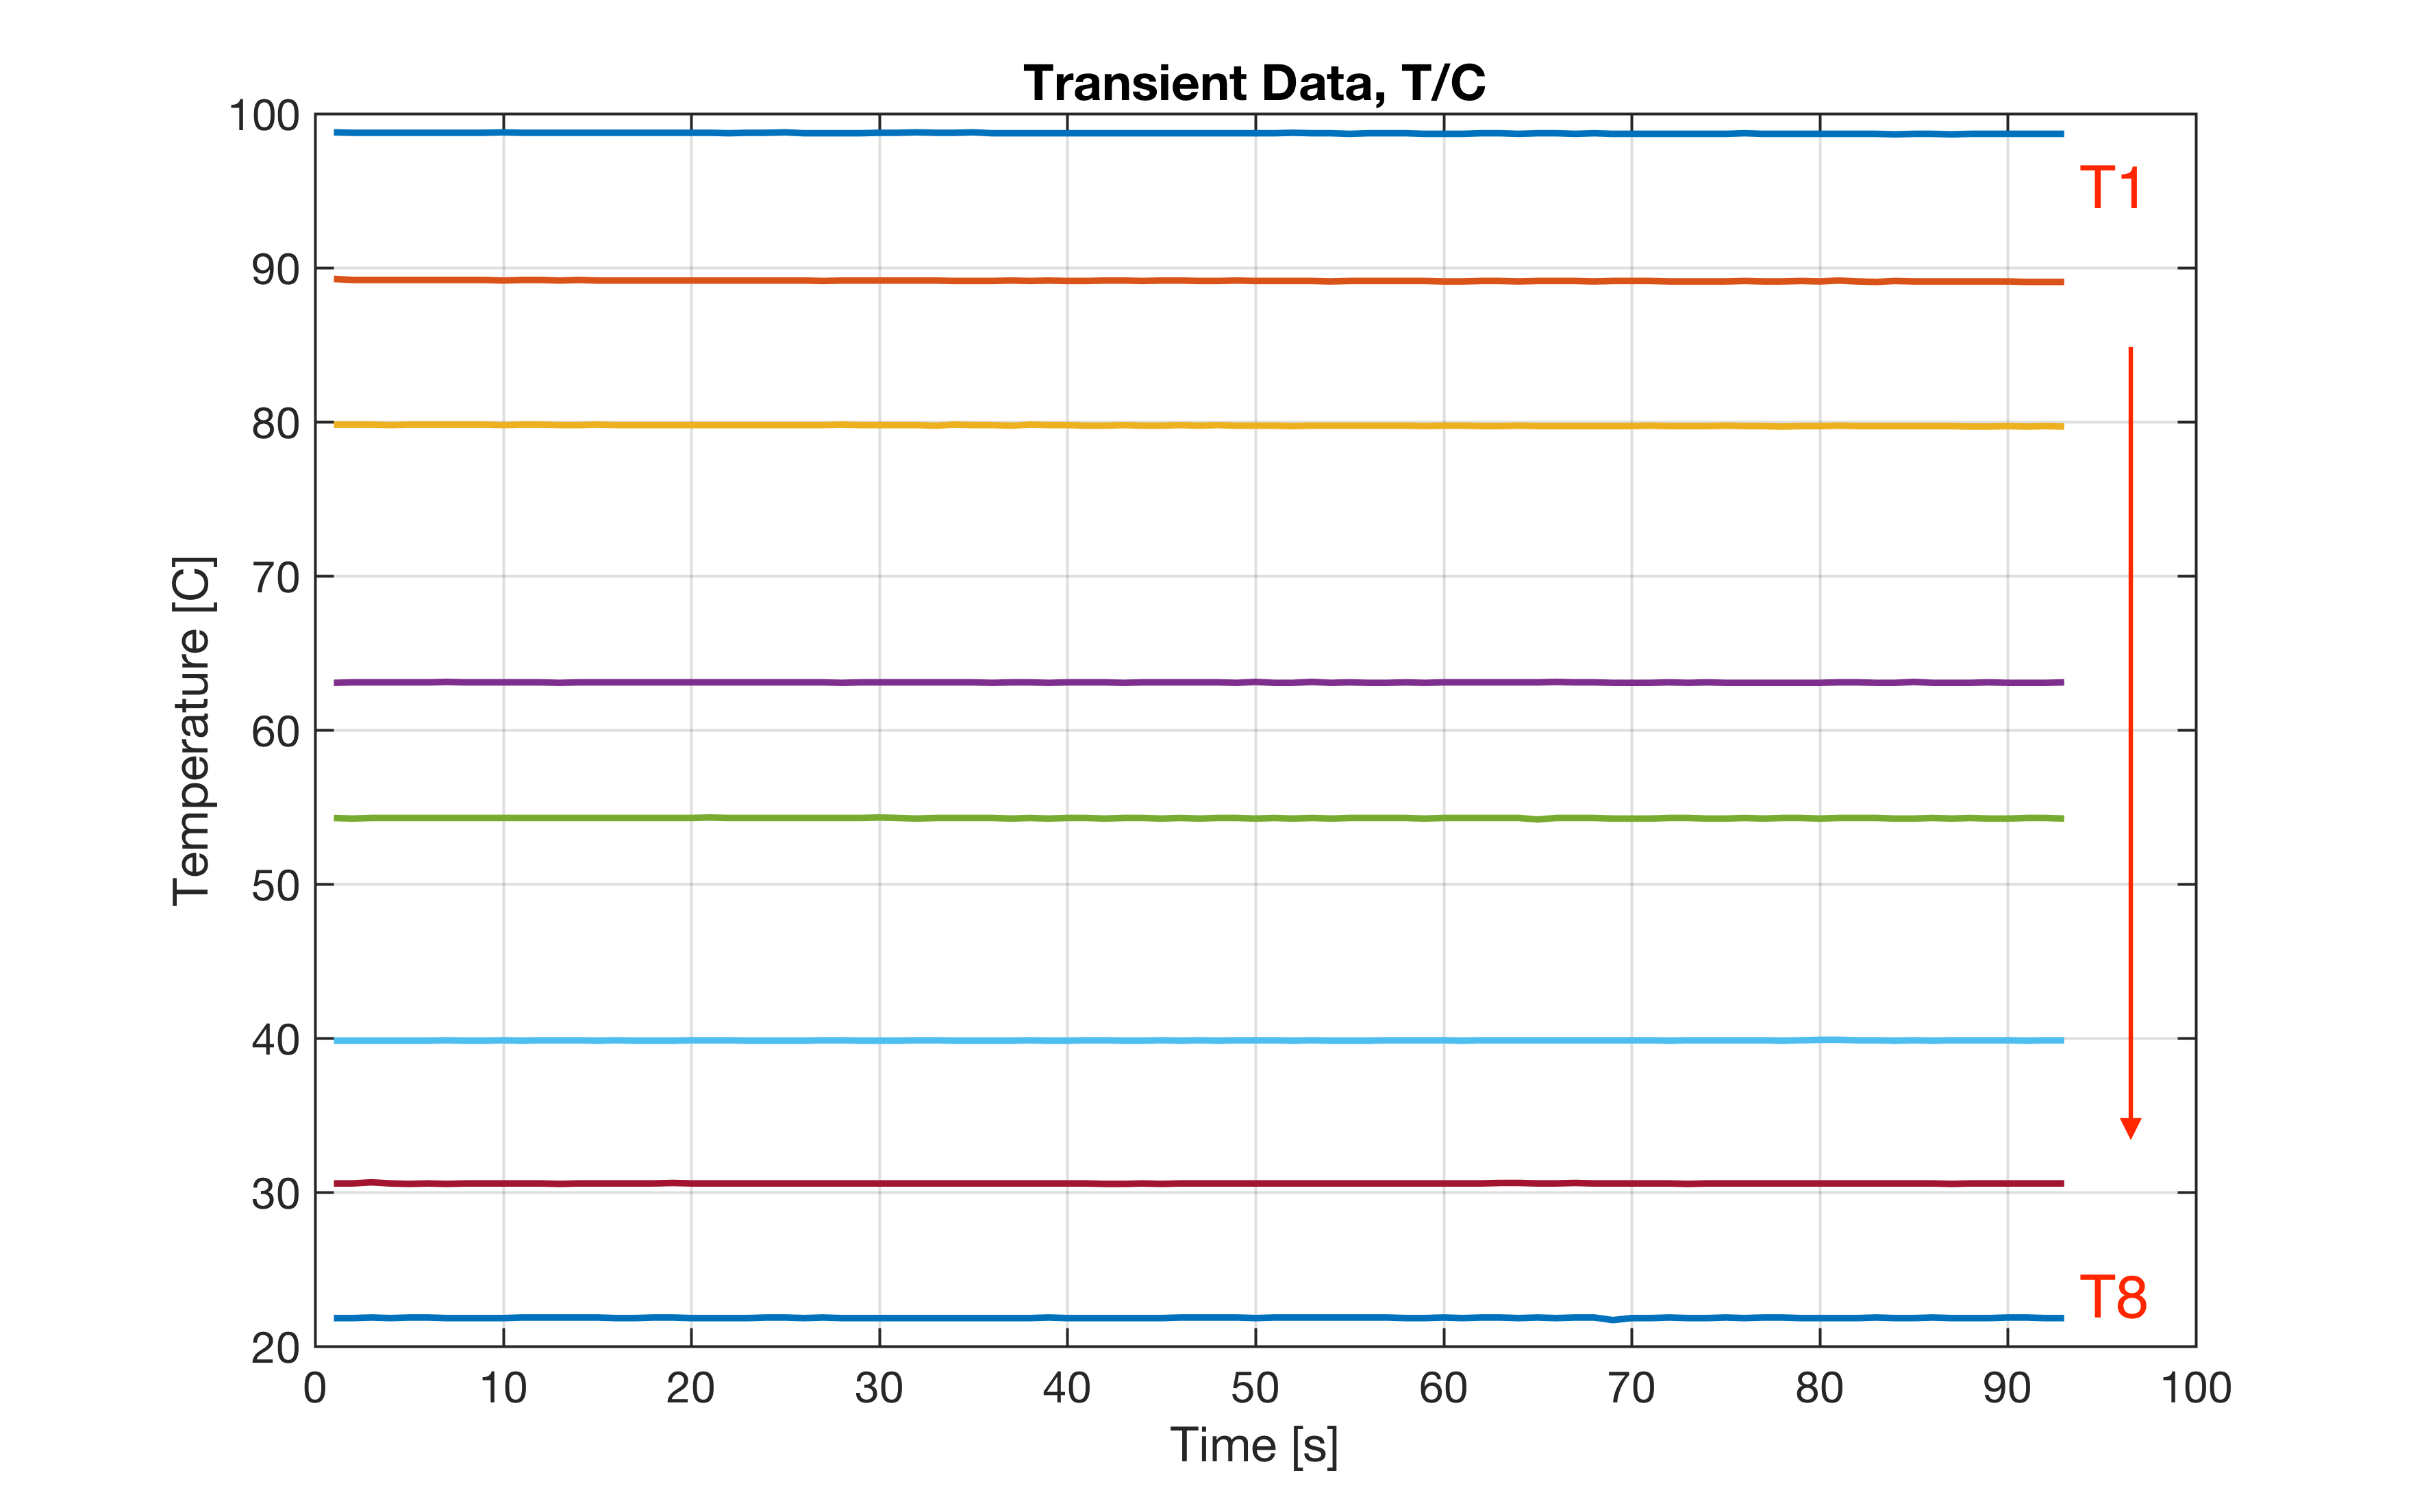
\includegraphics[width=125mm]{gfx/fig1.png}
    \caption{Transient temperature data}\label{fig1}
    \end{center}
\end{figure}

A few quick questions to ask:

\begin{formal}
\begin{quest} \bit{Sanity Check.}
\begin{itemize}
    \item Does your plot match Fig.~\ref{fig1} below? 
    \item \it{Are you using the correct version of \texttt{MATLAB}?} 
    \item Is all of our data at steady-state?
\end{itemize}
\end{quest}
\end{formal}
\begin{center}
\begin{tcolorbox}[enhanced, width=14cm, size=tight, top=-2mm, colback=red!5, colframe=black!50!white, boxrule=0.25pt, boxsep=2mm]
\n
{\small
\bit{Checkpoint} - If you had any difficulties obtaining Fig.~\ref{fig1}, \bul{stop here} and contact your Lab Instructor. You may run into more troubles ahead.
}
\end{tcolorbox}

\end{center}

When you're ready to continue, press \texttt{enter} to un-pause your program and proceed.

\n
\hrule

\section{Plot Data}

Now, let's actually plot the steady-state data. First,  we need to take an average of each column in $M$. This is done for you using the $mean( )$ command.

Then, we call a \texttt{plotData.m} function to plot our data. However, this plot function is incorrect and will not run correctly.  Therefore, you will need to do the following:
\begin{itemize}
    \item Open \texttt{plotData.m} 
    \item Adjust code accordingly to obtain Fig.~\ref{fig2} below.
\end{itemize}

\Note: if you program is paused, you may need to exit before opening \texttt{plotData.m}. This can be done by pressing \texttt{CTRL-C}.


\begin{figure}[H]
    \begin{center}
        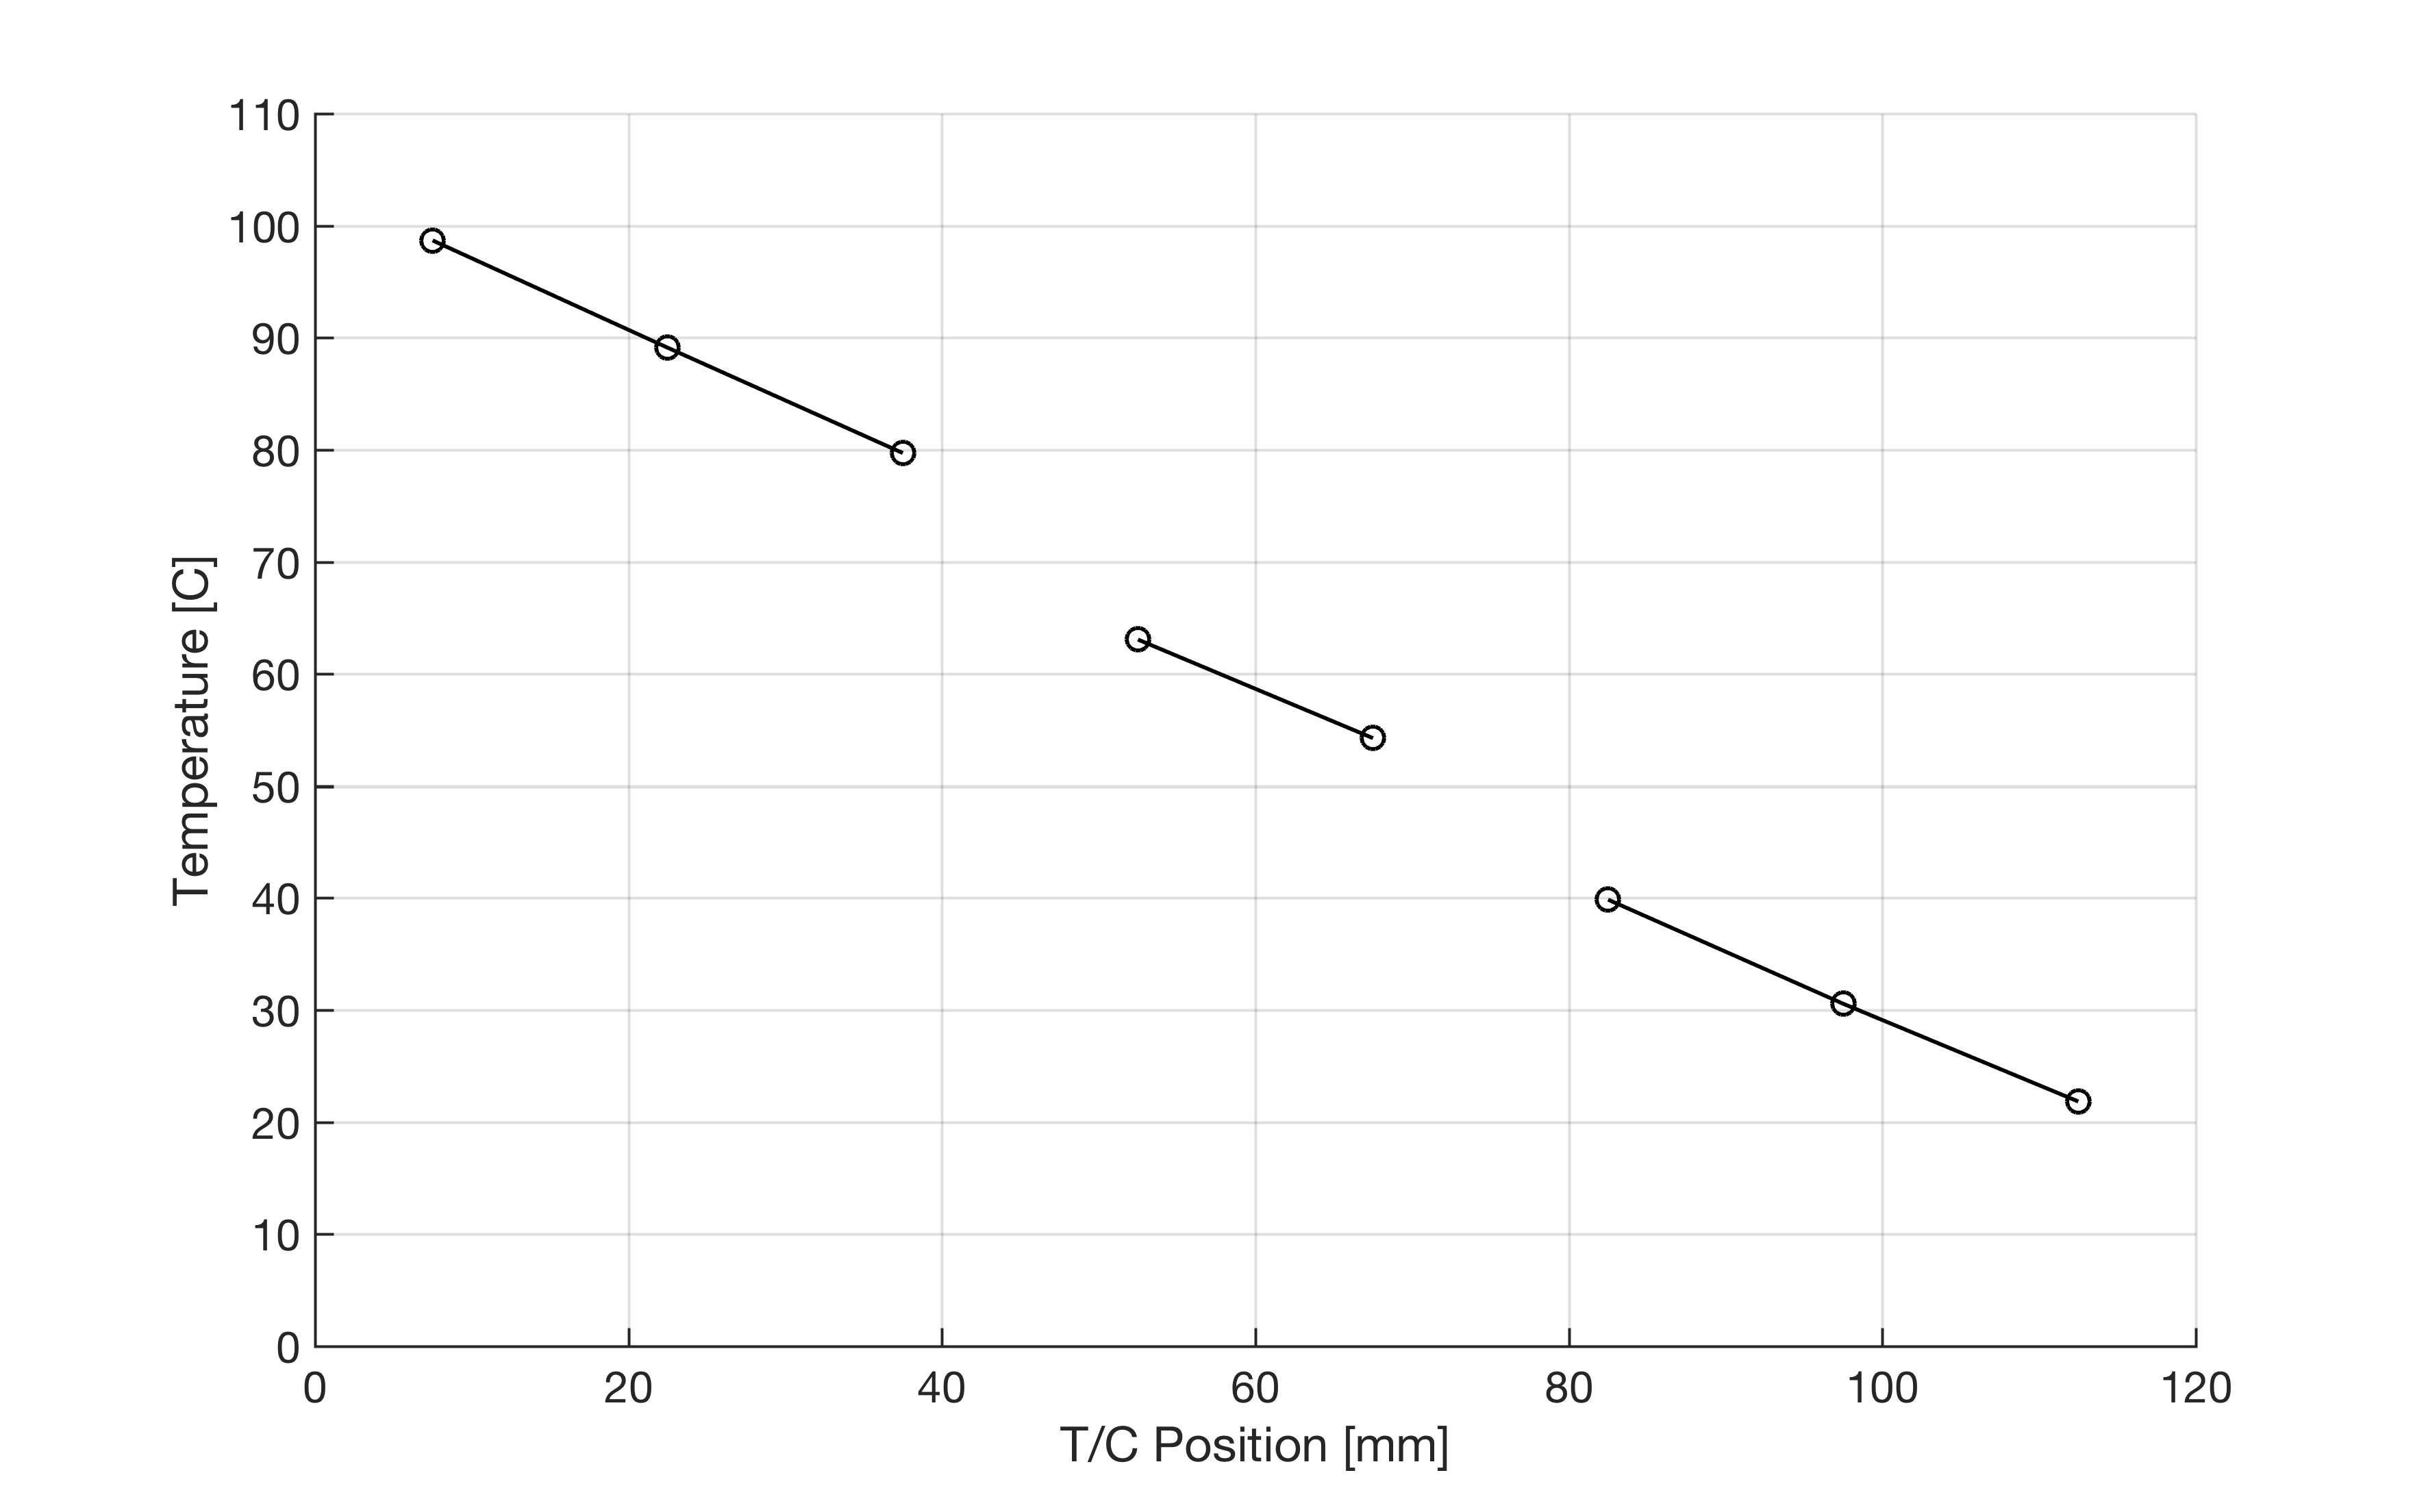
\includegraphics[width=125mm]{gfx/fig2.png}
    \caption{Transient temperature data}\label{fig2}
    \end{center}
\end{figure}

Then, if everything was done correctly in part 1a, you should be able to press \texttt{Enter} at the \texttt{pause} mark and arrive at a figure that resembles Fig.~\ref{fig3} below.

\begin{figure}[H]
    \begin{center}
        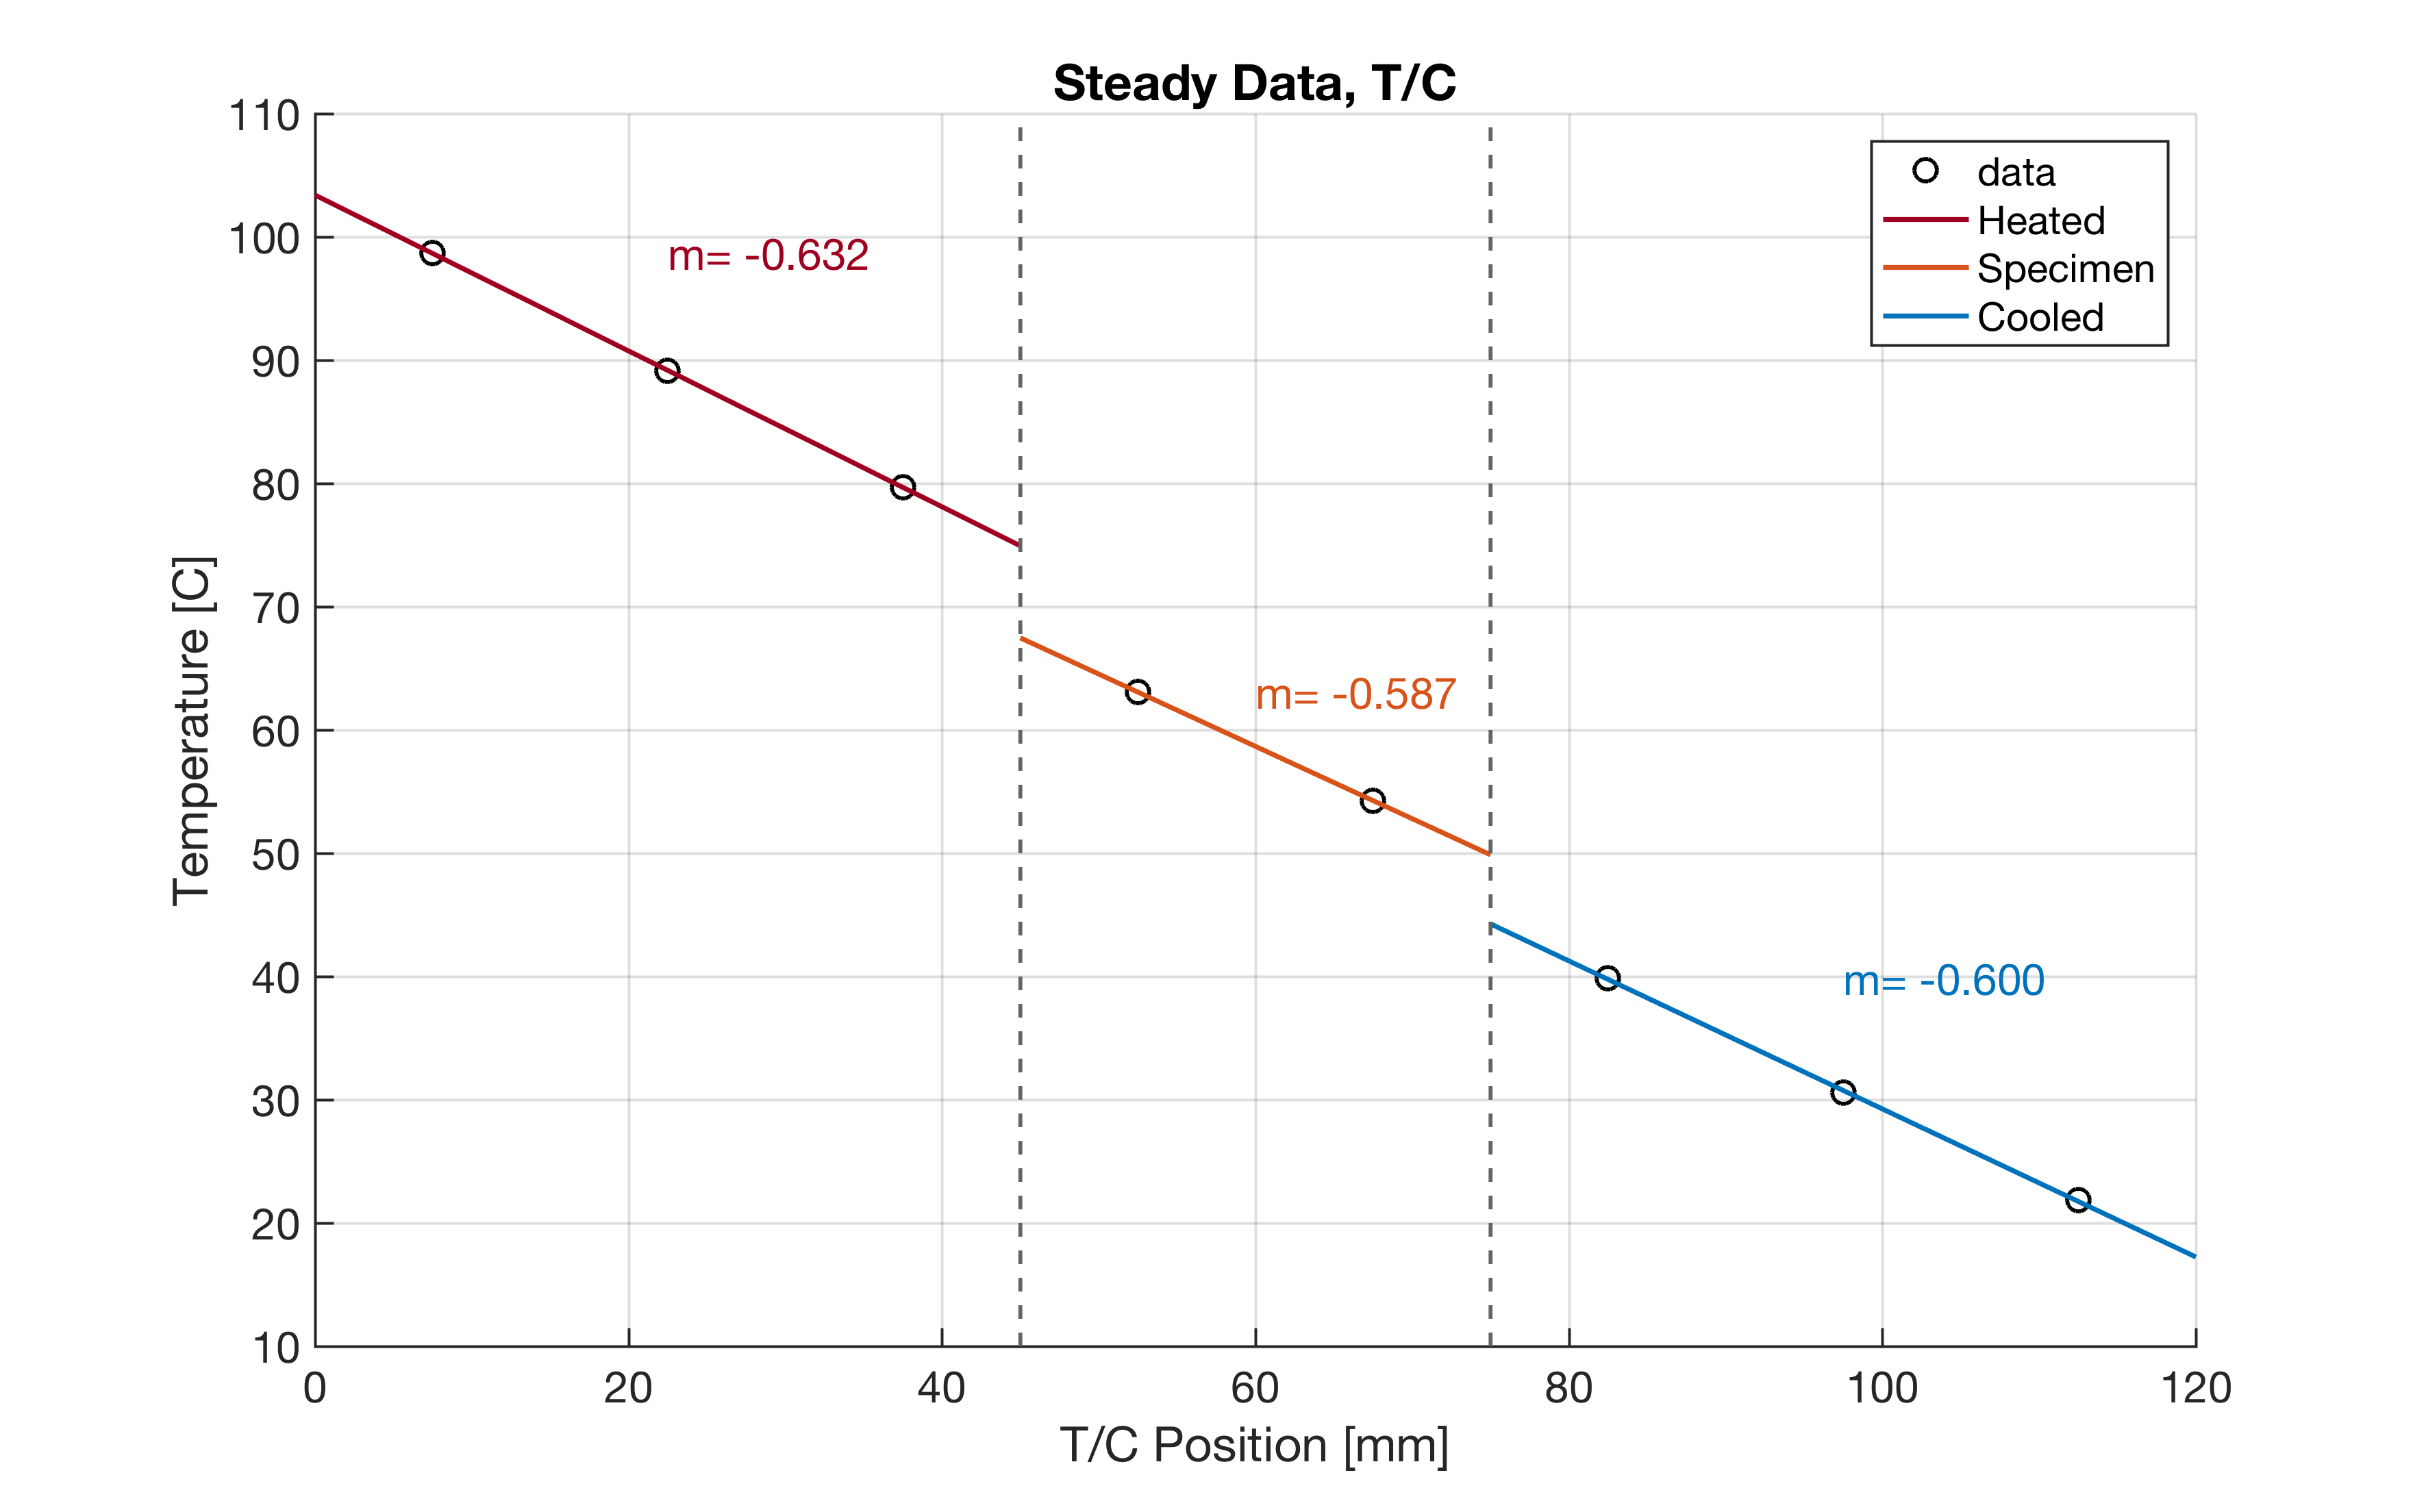
\includegraphics[width=125mm]{gfx/fig3.png}
    \caption{Steady-state T/C data}\label{fig3}
    \end{center}
\end{figure}

Here, we have added regression lines as well as some labels that will make more sense when we get to Lab 1.

\n
The box below outlines the \it{deliverable} for the pre-lab assignment:

\begin{formal}
    \begin{deliv} \bit{SAMPLE:  Steady-state T/C plot} (Fig.~\ref{fig3} above) 
   Export your figure to an image: \texttt{File >> Export Setup >> Export}, and include it in your submission.
    \end{deliv}
\end{formal}


\section*{Submission}

Once all of the deliverables have been completed, you will simple place the output into a single document and hand it to your TA at the beginning of lab. More details will be provided on a lab-to-lab basis.



\end{document}
